\section{Séance 5}

\textbf{Graphes Hamiltoniens}

\subsection{Cycle hamiltonien et eulerien}
Pour quelle classe de graphes un tour eulérien est-il aussi hamiltonien? Peut-on en déduire une caractérisation des graphes qui sont à la fois eulériens et hamiltoniens?
\begin{solution}
\begin{itemize}
\item Pour les graphes connexes dont tous les noeuds sont de degré 2.
\item Pour avoir un graphe qui est à la fois eulérien et hamiltonien, il faut partir du cycle hamiltonien de base. Si on décide d'ajouter des arêtes, il faut respecter la condition ``garder le degré pair''. En effet, le cycle hamiltonien n'est pas spécialement le même que le cycle eulérien.
\end{itemize}
\end{solution}

\subsection{Problème du cavalier}
Le problème du cavalier était un problème en vogue au XVIIIème siècle. Le problème est de déterminer s'il est possible de faire parcourir toutes les cases d'un échiquier de taille $n \times n$ à un cavalier en ne passant qu'une seule fois par chaque case et en revenant à son point de départ. Formulez cela comme un tour hamiltonien dans un graphe et montrez que la réponse est négative pour $n$ impair.
\begin{solution}
\subsection{Solution de Nicolas Stevens}
Chaque noeud représente une case de l'échiquier. Les arrêtes sont les déplacements possibles en partant d'une case. L'objectif est alors de trouver une cycle hamiltonien sur ce graphe. Pour le cas où $n$ est impair, on peut tirer parti d'une propriété de ce graphe : on remarque facilement que le graphe est biparti. Or si $n$ est impair, les deux partition des noeud sont de taille différentes. Dés lors il n'est pas possible de trouver un cycle qui parcourt tout les noeuds une et une seule fois et qui revient au point de départ.

\subsection{Solution de Félicien Schiltz}
Ce problème correspond à trouver un tour hamiltonien dans un graphe dans lequel les sommets sont les cases du graphe. Les sommets sont reliés entre eux lorsque le cavalier peut se déplacer d'un à l'autre directement.\\
Comme le mouvement du cavalier lui permet de se déplacer uniquement d'une case blanche à une case noire et d'une case noire à une case blanche, ce graphe est biparti.
Si $n$ est impair, le nombre de cases est impair également et le problème demande donc de trouver un cycle hamiltonien de longueur impaire dans un graphe biparti. Hors, un graphe est biparti si et seulement si il ne contient aucun cycle de longueur impaire. Il est donc impossible de résoudre ce problème si n est impair.
\textit{\textsc{En bref: }Dans un graphe biparti, si le nombre de noeuds n'est pas le même des deux côtés, le graphe n'est pas hamiltonien.}
\end{solution}

\subsection{Théorème de Dirac}
Le théorème de Dirac affirme que si $d(v) > n/2$ pour tous les sommets $v \in V$ d'un graphe $G=(V,E)$, alors $G$ est hamiltonien. Donnez un graphe hamiltonien de $n$ sommets qui ne satisfait pas les conditions du théorème de Dirac. Donnez un graphe qui n'est pas hamiltonien et qui satisfait $d(v) \geq (n-1)/2$ pour tout $v \in V$.

\begin{solution}
\begin{itemize}
\item Graphe hamiltonien de 5 sommets ne satisfaisant pas les conditions du théorème de Dirac.\\
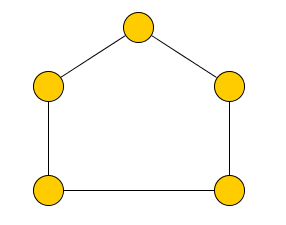
\includegraphics[scale=0.5]{ape5_ex3_1.png}
\item Graphe non hamiltonien de 5 sommets satisfaisant $d(v) \geq (n-1)/2$ pour tout $v \in V$.\\
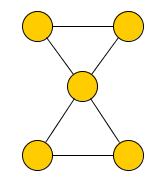
\includegraphics[scale=0.5]{ape5_ex3_2.png}
\end{itemize}
\end{solution}

\subsection{Double cycle hamiltonien}
Placez $n$ sommets sur un cercle et liez un sommet à ses deux plus proches voisins dans les deux directions. Démontrez que pour $n \geq 5$ le graphe obtenu est l'union de deux circuits hamiltoniens.

\begin{solution}
Pour $n$ impair, ce résultat est évident. On a le circuit hamiltonien intérieur (en vert) et celui extérieur (en rouge).\\
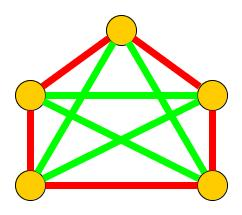
\includegraphics[scale=0.5]{nimpair.jpg}
\\
Pour $n$ pair, on propose une méthode de construction des 2 circuits hamiltoniens qui fonctionne pour tout $n$ pair. On commence par construire, pour $n=6$ le graphe suivant, avec le circuit hamiltonien intéreur (en vert) et celui extérieur (en rouge).
\\
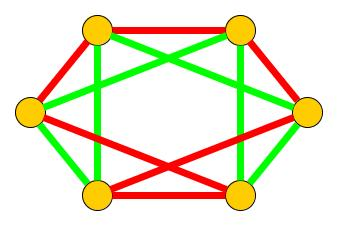
\includegraphics[scale=0.5]{npair1.jpg}
\\
Il est très facile d'ajouter les noeuds par 2 en complétant les circuits hamiltoniens. On construit d'abord le circuit extérieur (en rouge) en gardant toujours la même façon de procéder, et ensuite celui intérieur, qui comprend les arêtes non-utilisées par le circuit rouge. Voici le graphe pour $n=8$.
\\
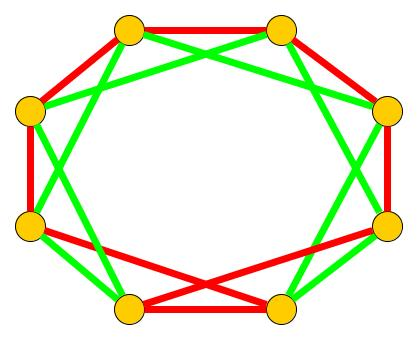
\includegraphics[scale=0.5]{npair2.jpg}
\\
\end{solution}

\subsection{Souris VS gruyère}
Une souris mange un gruyère de dimension $3 \times 3 \times 3$ par petits morceaux de taille $1 \times 1 \times 1$. Elle démarre en un coin du cube et se déplace de cube adjacent en cube adjacent. Peut-elle manger la totalité du gruyère en terminant par le cube central?
\begin{solution}
La justification est la même que pour le problème du cavalier. Modélisons le fromage comme un graphe dont chaque cube de dimension $1 \times 1 \times 1$ est un noeud et dont les noeuds représentant des cubes adjacents sont reliés par une arête.\\
En effet, ce graphe est biparti. On peut imaginer peindre le noeud de départ en blanc, ceux qui y sont adjacents en noir, ceux adjacents à ceux-ci en blanc etc.\\
Le nombre de noeuds peints en blanc sera donc 14 et ceux peints en noir 13. Il est évidemment impossible de trouver un chemin hamiltonien partant d'un coin (blanc) et se terminant au centre (noir) et ayant parcouru tous les noeuds.
\end{solution}

\begin{solution}
Chaque noeud représente une part du cube (27 parts au totale). Les arrêtes sont verticales ou horizontales. Ce faisant on a construit un graphe biparti. Comme il y a 27 noeuds, la bi-partition comporte respectivement 14 et 13 noeuds. Il n'est alors pas possible de construire un cycle qui passe par tous les noeuds et qui revient au point de départ. Une autre manière de voir les choses est d'utiliser la condition nécessaire sur les graphe hamiltoniens: si on supprime les 13 noeuds, on obtient 14 composantes connexes. Or si un graphe est hamiltonien, supprimer $k$ noeuds crée au plus $k$ composantes connexes. On a une contradiction et donc le graphe n'est pas hamiltonien.
\end{solution}

\subsection{Borne d'un voyageur de commerce}
Trouvez des bornes supérieures et inférieures sur la valeur optimale du problème du voyageur de commerce avec les distances suivantes (les distances satisfont l'inégalité triangulaire) :
\begin{equation}
  \left( \begin{matrix}
      - & 5 & 4 & 3 & 6 \\
      - & - & 6 & 4 & 5 \\
      - & - & - & 3 & 3 \\
      - & - & - & - & 5 \\
      - & - & - & - & -
  \end{matrix}  \right)
\end{equation}
\begin{solution}
Une borne supérieure de la solution optimale est obtenue en faisant par exemple le parcours 1-2-3-4-5: $5+4+3+6=18$\\
Une borne inférieure peut être obtenue en additionnant les 4 plus petites distances entre les villes: $3+3+4+4=12$\\
\end{solution}

\subsection{Ordonancement de taches sur une machine spécialisée}
Formulez le problème suivant comme le problème du voyageur de commerce. Cinq opérations $j=1,…,5$ doivent avoir lieu sur une machine spécialisée. Les temps de transition $c_{ij}$ entre deux opérations sont importants, et sont donnés dans la table suivante:
\begin{equation}
  \left( \begin{matrix}
      10 & 23 & 42 & 11 & 24 \\
      19 & 13 & 42 & 36 & 43 \\
      67 & 34 & 23 & 29 & 21 \\
      19 & 52 & 41 & 37 & 31 \\
      96 & 63 & 75 & 89 & 43
  \end{matrix}  \right)
\end{equation}
En plus, si une opération $j$ est en première position, il faut aussi un temps de préparation $t_j$ qui est fonction de l'opération, où $t=(23,41,32,54,11)$. Pour des raisons techniques, on décide que l'opération $3$ ne peut pas précéder directement l'opération $1$, et les opérations $4$ et $5$ ne peuvent pas avoir lieu en dernière position.

\begin{solution}
Ce problème peut être modélisé comme le problème du voyageur de commerce dans un graphe orienté.
\begin{itemize}
\item Les opérations (par lesquelles il faut toutes passer) représentent les villes et sont modélisées comme des noeuds. 
\item Les arêtes sont les temps de transitions entre les opérations et relient ces opérations en étant dirigées de l'opération de départ  celle d'arrivée. Leur poids est le temps de transition. Elles représentent les routes dans le problème du voyageur de commerce.
\item On ajoute un noeud de départ, qui est relié à toutes les opérations par des arêtes qui ont des poids valant les temps de préparations respectifs des opérations et en étant dirigées vers les opérations. 
\item On ajoute également un noeud d'arrivée, auquel sont reliées toutes les opérations à l'aide d'arêtes de poids nuls en étant dirigée vers ce noeud.
\item Afin de modéliser la condition ``L'opération 3 ne peut pas précéder directement l'opération 1'', on supprime l'arête partant de l'opération 3 et allant vers l'opération 1.
\item Afin de modéliser la condition ``les opérations 4 et 5 ne peuvent pas avoir lieu en dernière position'', on supprime les arêtes qui partent des opérations 4 et 5 sont dirigées vers le noeud d'arrivée
\end{itemize}
\end{solution}

\subsection{Diner en territoire ennemi}
Un groupe de huit personnes se retrouve pour diner. Le graphe ci-dessous précise les ``incompatibilités d'humeur'' entre les personnes de ce groupe (une arête reliant deux personnes indique que celles-ci s'entendent très modérément). Proposez un plan de table (la table est ronde) pour ce groupe en évitant de placer côte à côte deux personnes ``incompatibles''.

\begin{figure}[h!]
  \begin{center}
    \begin{tikzpicture}[-,>=stealth',shorten >=1pt,auto]
      \Vertex[x=0 ,y=0]{8}
      \Vertex[x=0 ,y=-2]{7}
      \Vertex[x=2,y=1]{1}
      \Vertex[x=2 ,y=-3]{6}
      \Vertex[x=4 ,y=1]{2}
      \Vertex[x=4 ,y=-3]{5}
      \Vertex[x=6 ,y=0]{3}
      \Vertex[x=6 ,y=-2]{4}


      \path[every node/.style={font=\sffamily\small}]
      (1) edge node [left] {} (2)
      edge node [left] {} (4)

      (2) edge node [right] {} (5)
      edge node [right] {} (6)
      edge node [right] {} (8)

      (3) edge node [right] {} (4)
      edge node [left] {} (5)

      (4) edge node [right] {} (7)

      (5) edge node [right] {} (6)

      (6) edge node [right] {} (8)

      (7) edge node [left] {} (8);

    \end{tikzpicture}
  \end{center}
\end{figure}

\begin{solution}
Afin de trouver un plan de table qui conviendrait, il faut d'abord créer le complémentaire du graphe précédent. Dans celui-ci, les arêtes relient deux personnes qui s'entendent bien. Il faut ensuite trouver un cycle hamiltonien dans ce graphe, et l'ordre dans lequel les noeuds sont parcourus sera celui dans lequel les gens sont placés autour de la table. Une solution possible est la suivante:$1-3-6-4-2-7-5-8$
\end{solution}

\newpage

\textbf{Couplages}

\subsection{Couplage maximum}
Etant donné le couplage $M = \left\lbrace  (1,1'), (2,4'),(4,2'),(5,5')  \right\rbrace$ dans le graphe biparti ci-dessous, démontrez que $M$ est maximum.

\begin{figure}[h!]
  \begin{center}
    \begin{tikzpicture}[-,>=stealth',shorten >=1pt,auto]
      \Vertex[x=0 ,y=0]{1}
      \Vertex[x=0 ,y=-1]{2}
      \Vertex[x=0,y=-2]{3}
      \Vertex[x=0 ,y=-3]{4}
      \Vertex[x=0 ,y=-4]{5}
      \Vertex[x=3 ,y=-0]{1'}
      \Vertex[x=3 ,y=-1]{2'}
      \Vertex[x=3 ,y=-2]{3'}
      \Vertex[x=3 ,y=-3]{4'}
      \Vertex[x=3 ,y=-4]{5'}


      \path[every node/.style={font=\sffamily\small}]
      (1) edge [style=dashed]  node [left] {} (1')
      edge node [left] {} (5')

      (2) edge node [right] {} (1')
      edge node [right] {} (2')
      edge node [right] {} (3')
      edge [style=dashed]  node [right] {} (4')
      edge node [right] {} (5')

      (3) edge node [right] {} (1')
      edge node [left] {} (5')

      (4) edge [style=dashed]  node [right] {} (2')
      edge node [right] {} (3')
      edge node [right] {} (4')
      edge node [right] {} (5')

      (5) edge node [right] {} (1')
      edge [style=dashed]  node [left] {} (5');


    \end{tikzpicture}
  \end{center}
\end{figure}
\begin{solution}
Un couplage dans un graphe est un ensemble M d’arêtes tel que
M ne contient pas de boucles et deux arêtes de M n’ont jamais
d’extrêmité en commun. Hors, les seuls noeuds qui ne sont pas encore des extrémités dans ce couplage M sont les noeuds $3$ et $3'$. Si M est maximum, on ne peut pas lui ajouter d'arête. Hors la seule arête qu'on pourrait lui ajouter serait une qui relie les noeuds $3$ et $3'$. Cette arête n'existant pas dans ce graphe, M est bien maximum.
\end{solution}

\subsection{Vrai ou faux}

\begin{itemize}
  \item Un arbre possède un couplage parfait si et seulement si tous les chemin d'une feuille à une autre sont de longueur impaire.
  \item Un arbre possède au plus un couplage parfait.
  \item Dans un arbre, si pour tout noeud $u$, il existe une feuille $v$ telle que $d(u,v)$ est impaire, alors cet arbre possède un couplage parfait.
  \item Soit $o(H)$, le nombre de composantes impaires du graphe $H$, c'est-à-dire le nombre de composantes connexes ayant un nombre impair de sommets. Un arbre $G$ admet un couplage parfait si $o(G-v)=1,  \ \ \forall v \in V$.
  \item Si un arbre $G$ admet un couplage parfait, alors $o(G-v)=1, \ \ \forall v \in V$.
\end{itemize}


\subsection{Assistanat INMA}
Thibault a la responsabilité de répartir les séances d'exercices des cours de mathématiques appliquées entre les assistants du pôle INMA. Chacun des assistants donne pour cela à Thibault une liste de ses cours préférés, qui sont repris dans la table ci-dessous.

\begin{center}
  \begin{tabular}{|c|c|}
    \hline
    Assistant & Cours préférés \\
    \hline
    Pierre & Projet, Théorie des Matrices \\
    Romain & Graphes, Modélisation Stochastique \\
    Arnaud & Théorie des Matrices \\
    Adeline & Graphes, Optimisation, Analyse Numérique \\
    Benoit & Théorie des Matrices, Projet \\
    Nicolas & Graphes, Optimisation, Analyse Numérique, \\
            & Modélisation Stochastique, Théorie des Matrices  \\
    \hline
  \end{tabular}
\end{center}

Thibault aimerait bien assigner exactement un cours à chaque assistant en respectant autant que possible leurs préférences. Formulez cela comme un problème de couplage maximum dans un graphe.

Pour l'aider dans sa tâche, Thibault dispose de la répartition de l'année dernière:

\begin{center}
  \begin{tabular}{|c|c|}
    \hline
    Romain & Modélisation Stochastique \\
    Adeline & Optimisation \\
    Nicolas & Théorie des Matrices \\
    Pierre & Projet \\
    \hline
  \end{tabular}
\end{center}

En partant de la répartition de l'année dernière, utilisez l'algorithme hongrois pour aider Thibault à trouver un couplage maximum. Ce couplage est-il parfait? Proposez un argument pour prouver que le couplage trouvé est effectivement maximum.




%Dans le graphe graphe biparti ci-dessous, un couplage possible est $M = \left\lbrace  (1,5'), (2,2'),(3,6'),(5,4')  \right\rbrace$. En partant de ce couplage, utilisez l'algorithme hongrois pour trouver un couplage maximum. Proposez un argument pour prouver que le couplage trouvé est effectivement maximum.

%\begin{figure}[h!]
%\begin{center}
%\begin{tikzpicture}[-,>=stealth',shorten >=1pt,auto]
%   \Vertex[x=0 ,y=0]{1}
%   \Vertex[x=0 ,y=-1]{2}
%   \Vertex[x=0,y=-2]{3}
%   \Vertex[x=0 ,y=-3]{4}
%   \Vertex[x=0 ,y=-4]{5}
%   \Vertex[x=0, y=-5]{6}
%   \Vertex[x=3 ,y=-0]{1'}
%   \Vertex[x=3 ,y=-1]{2'}
%   \Vertex[x=3 ,y=-2]{3'}
%   \Vertex[x=3 ,y=-3]{4'}
%   \Vertex[x=3 ,y=-4]{5'}
%   \Vertex[x=3, y=-5]{6'}
%
%     \path[every node/.style={font=\sffamily\small}]
%     (1) edge  node [left] {} (1')
%        	edge [style=dashed]  node [left] {} (5')
%
%    (2) edge node [right] {} (1')
%    	edge [style=dashed]  node [right] {} (2')
%    	edge node [right] {} (3')
%
%    (3) edge node [right] {} (1')
%     	edge  node [right] {} (2')
%    	edge node [right] {} (3')
%         edge  node [left] {} (5')
%         edge [style=dashed]  node [left] {} (6')
%
%    (4) edge node [right] {} (6')
%
%     (5) edge [style=dashed] node [right] {} (4')
%         edge node [left] {} (6')
%
%     (6) edge node [right] {} (4')
%         edge  node [left] {} (6')
%
%
%\end{tikzpicture}
%\end{center}
%\end{figure}


\subsection{Gagner sans le couplage parfait}
Deux personnes jouent à un jeu sur un graphe $G$ de la manière suivante: \\

\begin{itemize}
  \item Chacune des deux personnes sélectionne chacune à son tour un sommet $v_1, v_2, v_3, …$ tel que $\forall i > 1, \ \ \ v_i$ est adjacent à $v_{i-1}$.
  \item Un sommet déjà sélectionné ne peut plus être choisi.
  \item La dernière personne à sélectionner un sommet gagne le jeu.
\end{itemize}

Montrer que le premier joueur admet une stratégie gagnante si et seulement si le graphe $G$ n'admet pas de couplage parfait.
